\chapter{Updates to the Noise Simulation}
The search for tau neutrinos is a search for rare particles near the detector threshold.
Under these conditions, the search requires excellent understanding of threshold effects and detector behavior.
In order to better model the detector, the noise simulation used in IceCube was updated with improved measurements after the discovery of disagreements in charge variables.
This process is described in this chapter.

The chapter begins by describing the process used in previously to fit the Vuvuzela noise model for each DOM in Section~\ref{sec:old_vuvuzela}.
The limitations of the previous fitting process and the discovery of new disagreements is discussed in Sections~\ref{sec:vuvuzela_limitations} and \ref{sec:lowdt_vuvuzela} respectively.
The new fitting procedure is then described in Section~\ref{sec:vuvuzela_fitting}.
New results of the fitting procedure are then discussed in Section~\ref{sec:vuvuzela_newfits}.

\label{sec:old_vuvuzela}
\section{A Summary of Previous Fits}
Detector noise is a nuisance in most physics and astronomy experiments.
PMT noise is assumed to be due to random emission from the photocathode and is affected by the gain of the PMT.
Noise pulses from PMTs appear uniformly in time as a Poisson process.

The Poissonian noise model was used in the past in IceCube. 
With the introduction of the lower trigger threshold in DeepCore in 2010, however, it became clear that additional unsimulated sources of noise exist \cite{Thesis-Vuvuzela}.
These additional hits appeared to occur in 'bursts' on a single PMT extending for up to a millisecond.
Due to the time-correlations of these hits, the phenomenon was labeled \emph{correlated noise}.

The Vuvuzela model, described briefly in Section~\ref{subsec:noise}, is now used to model both the Poissonian and non-Poissonian noise in IceCube.
The empirical model consists of a Poisson process for electronic noise and radioactive decays and a correlated component modeled with a log-normal distribution.
The model contains five free parameters per DOM.
Ten minutes of untriggered data from the detector, dominated by noise hits, was used for calibration of the Vuvuzela parameters.

The Vuvuzela noise model is fit using the distributions of the time between subsequent hits, shown previously in Figure~\ref{fig:noise_model}.
Fits for each DOM were performed using the Pearson chi-squared test statistic between the data histogram, $d$, and the simulated histogram, $m$.

\begin{equation}
\chi^2 = \sum_i^{bins} \frac{\left(d_i-m_i\right)^2}{m_i}
\end{equation}

\begin{figure}[h]
\centering
\begin{tabular}[b]{c}
  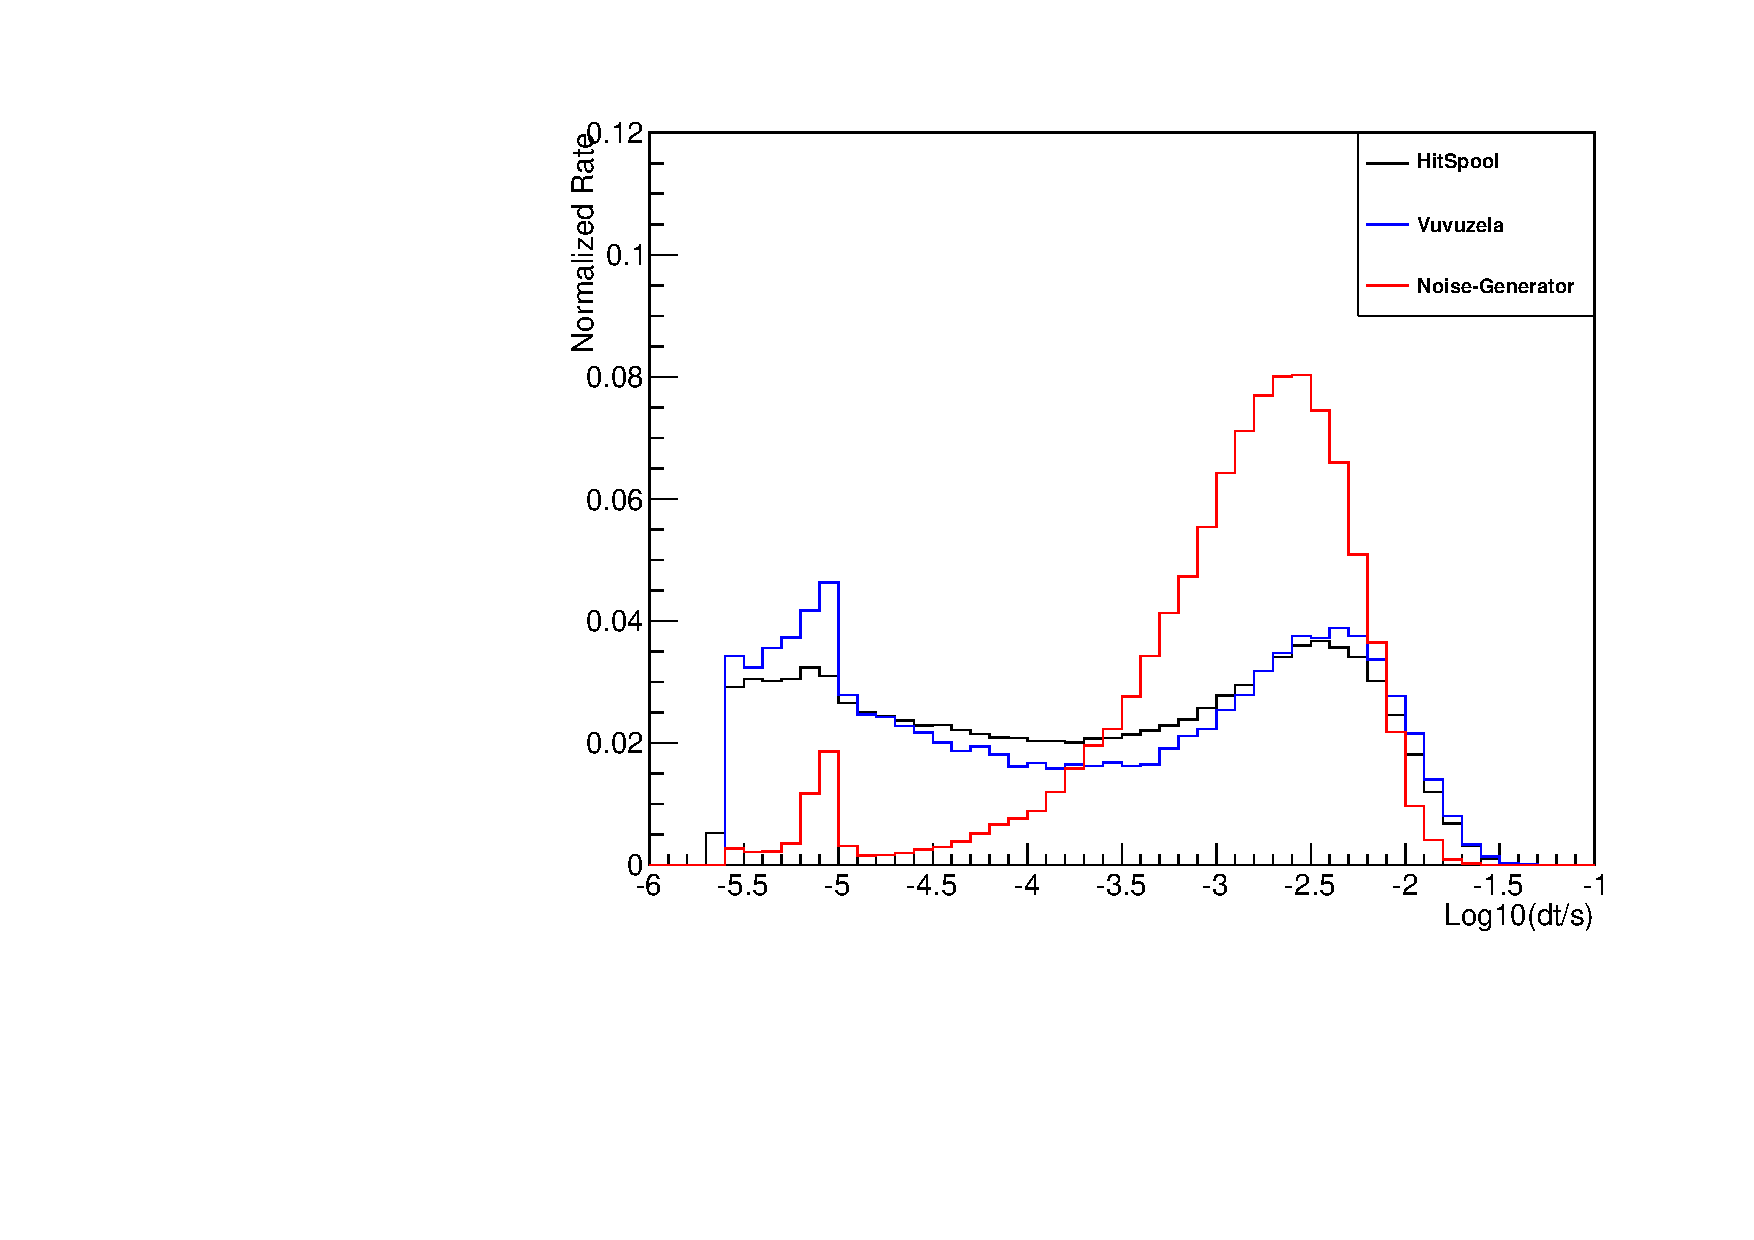
\includegraphics[width=0.45\linewidth]{old_dom_11-19.pdf} \\
  \small (\textbf{\color{ctcolormain}a}) DOM 11-19
\end{tabular} \hspace{2pt}
\begin{tabular}[b]{c}
  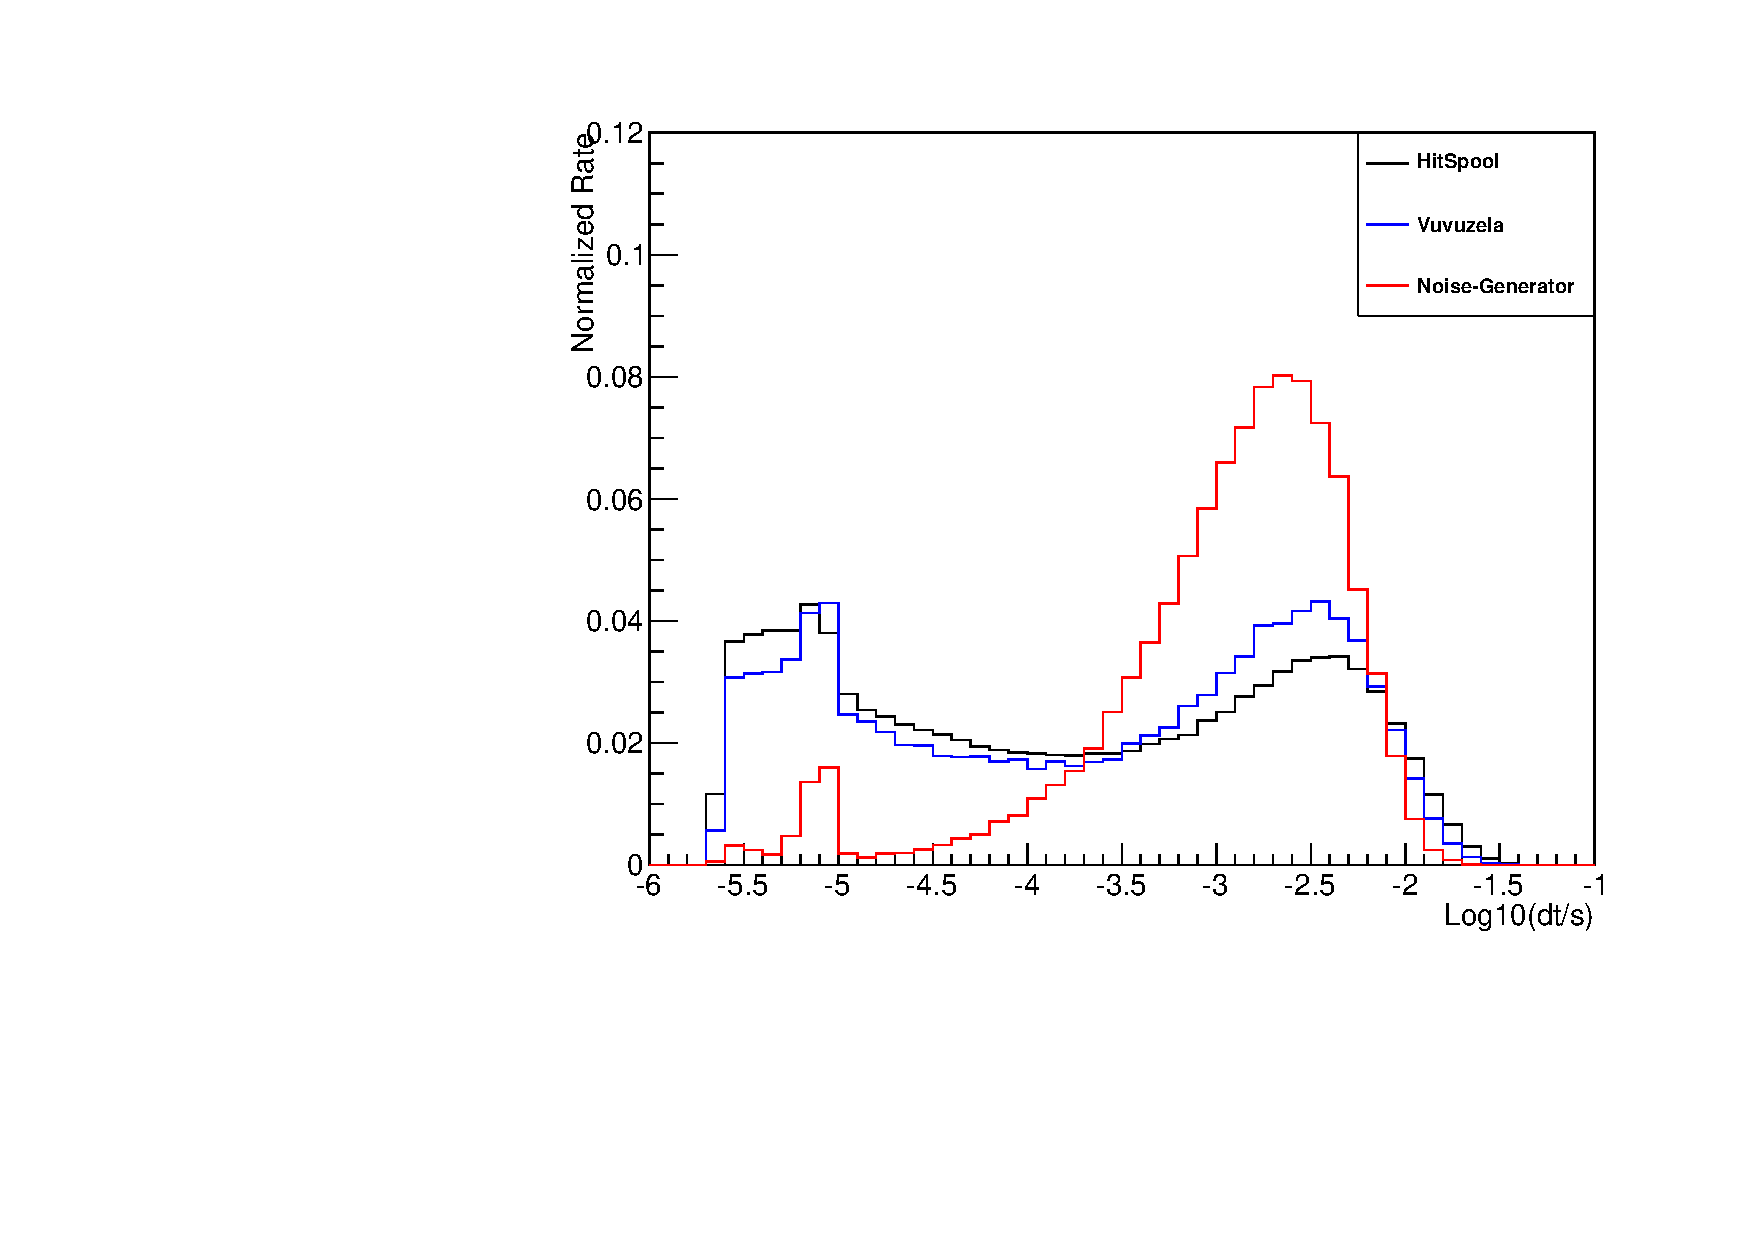
\includegraphics[width=0.45\linewidth]{old_dom_83-42.pdf} \\
  \small (\textbf{\color{ctcolormain}b}) DOM 83-42
\end{tabular}
\caption{Two examples of the original calibration work for the Vuvuzela model. The distribution of the time ("dt") between hits is shown. In black, untriggered detector data is shown. In red, a purely Poissonian noise model is shown. An afterpulsing peak is visible at $10^{-5}$ s. The Vuvuzela model is shown in blue. The Vuvuzela model shows improved agreement with data at all timescales.}
\label{fig:old_vuvuzela_fits}
\end{figure}


The value of the $\chi^2$ was minimized using a Metropolis-Hastings algorithm \cite{PDG-2015}.
For each iteration of the algorithm, new parameters were selected and the response of the DOM was resimulated using PMTResponseSimulator and DOMLauncher.
Each fit was computationally intensive, requiring between two and four CPU-weeks for each DOM.
Due to the computationally requirements of the fits, the stopping condition was intentionally loosely defined, with a goodness-of-fit of 10\% used.

\begin{figure}
\centering
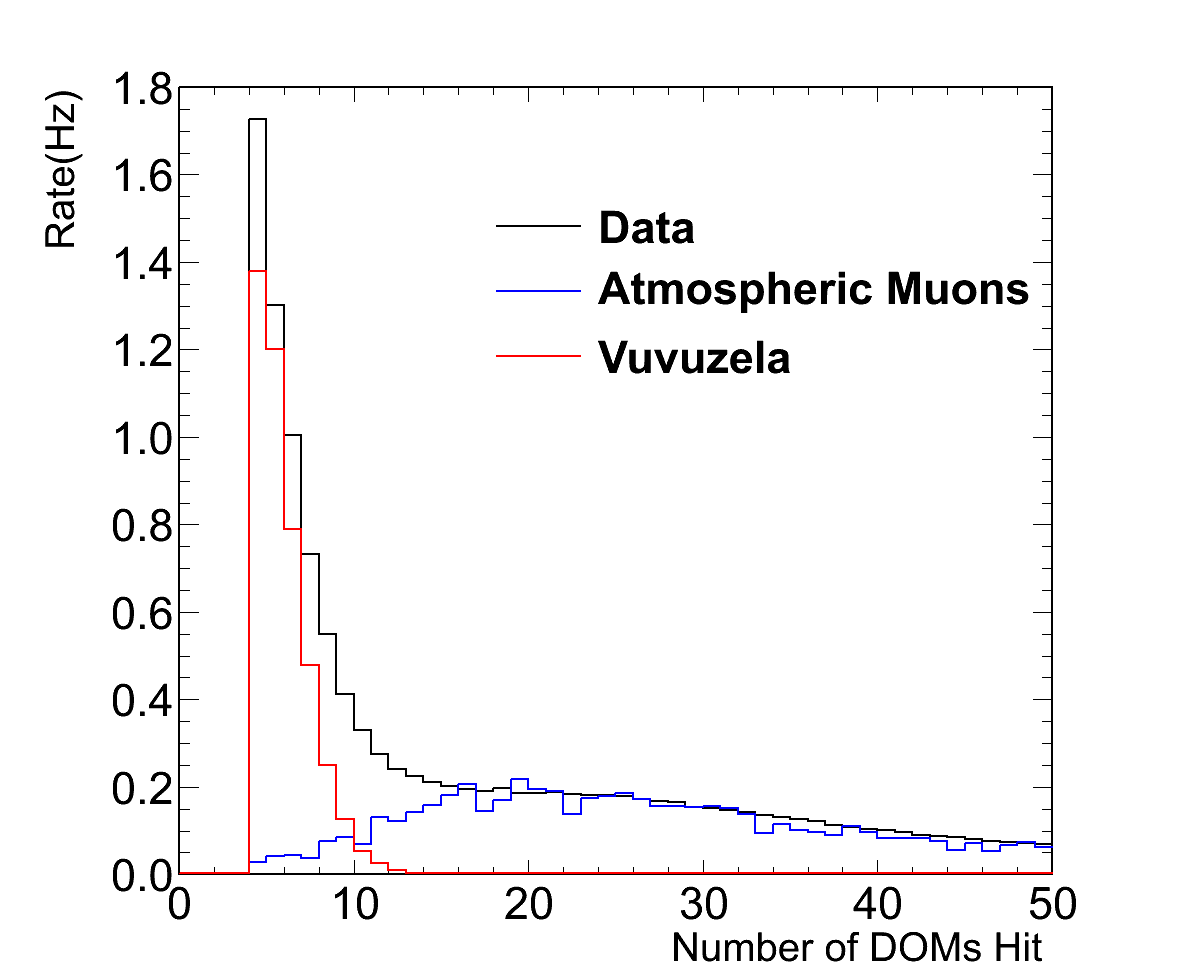
\includegraphics[width=0.6\textwidth]{srtwofflinepulsesdc_withnoise_vuvuzela.png} 
\caption{The rates of events in DeepCore as a function of the number of hit DOMs in a cleaned hit series. The data, shown in black, consists of two components: the accidental triggers (red) and the atmospheric muons (blue). Accidental triggers produced using the Vuvuzela noise model reproduce most of the rate of events below 10 hit DOMs, although a rate disagreement remains. Image from \cite{Thesis-Vuvuzela}.}
\label{fig:old_nch}
\end{figure}

Two examples from the original calibration work are shown in Figure~\ref{fig:old_vuvuzela_fits}.
The Poissonian noise model used previously is shown for comparison.
The Vuvuzela model more accurately reproduces the observed data across all timescales.
Distributions of the number of hit DOMs and the number of accidental triggers due to detector noise, shown in Figure~\ref{fig:old_nch}, improve significantly after inclusion of the updated noise model \cite{Thesis-Vuvuzela}.

\label{sec:vuvuzela_limitations}
\section{Limitations and Disagreement with Previous Fits}
While accidental triggers with the Vuvuzela model better reproduced the rates observed in data, Figure~\ref{fig:old_nch} showed disagreement between data and simulation at very low numbers of hits.
This region of the parameter space is dominated by accidental noise triggers in simulation.

An evaluation of the limitations of the previous calibration was performed in 2014, uncovering a number of possible improvements.
The original fits were limited due to a number of factors. 
For example, the fits excluded the effect of atmospheric muons in the detector under the assumption that the hit rate per DOM due to atmospheric muons (approximately 5 Hz) is significantly smaller than the noise hit rate observed in previous calibration (about 600 Hz).
Potential issues may arise from this assumption, which was not tested during original calibrations, including any potential time-correlated hits associated with muons.

Furthermore, some fits resulted in potentially-incomplete minimization.
Due to the nature of the fit distributions, there existed significant degeneracy in the parameter space, leading to further difficulties.

During the fitting process, the strength of the afterpulsing peak at 9 microseconds was discovered to differ between DOMs.
This effect was unsimulated, leading to convergence problems when fitting this region.
In response, fits were artificially limited to timescales longer than 10 microseconds, allowing the minimizer to only observe part of the correlated noise distribution.

Because the noise hits are unlikely to satisfy the HLC conditions, timescales smaller than 6.4 microseconds were unavailable for investigation.
No checks were performed for the Vuvuzela model below this limit..
The noise model itself was used down to 2 microseconds, however, resulting in uncertainty due to the extrapolation of the noise model to shorter times.
The limit of 2 microseconds was implemented due to the inherent difficulty in characterizing effects at these timescales due to artificial deadtime related to the HLC launch readout. 

\label{sec:lowdt_vuvuzela}
\section{Low-dt Noise from Vuvuzela}
In an attempt to address the imposed simulation limit at 2 microseconds, a new version of the Vuvuzela code, was created with this cutoff removed.
The resulting noise, labeled \emph{low-dt} noise for the short timescales ($\Delta$t), was used to produce a simulation of accidental noise triggers and CORSIKA muons for testing without further calibration.

\begin{figure}[h]
\centering
\begin{tabular}[b]{c}
  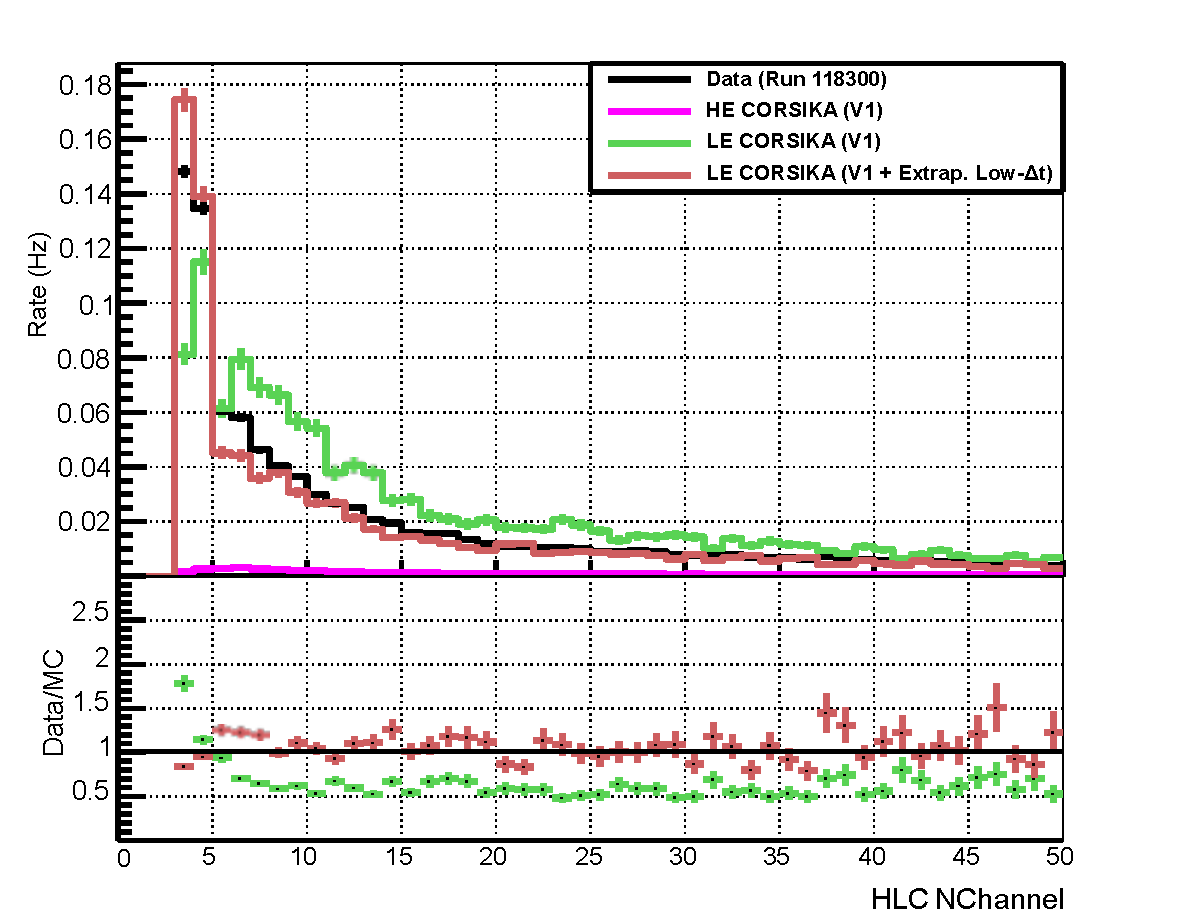
\includegraphics[width=0.45\linewidth]{old_HLC_NChannel.pdf} \\
  \small (\textbf{\color{ctcolormain}a}) HLC hits in DeepCore Events
\end{tabular} \hspace{2pt}
\begin{tabular}[b]{c}
  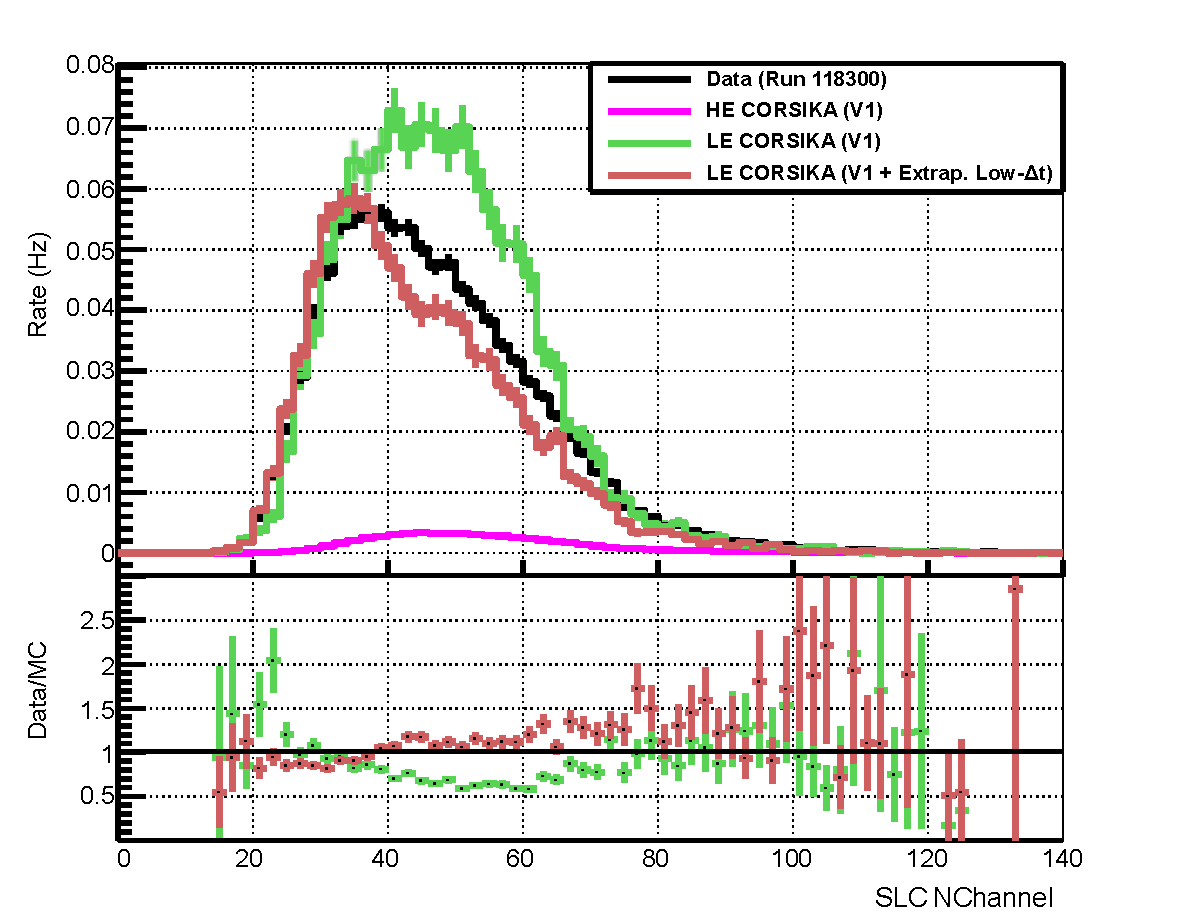
\includegraphics[width=0.45\linewidth]{old_SLC_NChannel.pdf} \\
  \small (\textbf{\color{ctcolormain}b}) SLC hits in DeepCore Events
\end{tabular}
\caption{The number of hit DOMs satisfying the (a) HLC and (b) SLC criteria described in Section~\ref{subsec:LC}. The distribution from 8 hours of data (black) is shown compared to a sample of CORSIKA muons at low-energy (600 GeV $\leq E_{primary} \leq$ 100 TeV) and high energy (100 TeV $\leq E_{primary} \leq$ 100 EeV). The addition of the low-dt extension to Vuvuzela improves the agreement between data and simulation in both HLC and SLC distributions.}
\label{fig:uncalibrated_nchannel}
\end{figure}

The first tests, shown in Figure~\ref{fig:uncalibrated_nchannel}, used the number of hit DOMs in DeepCore events to evaluate the effect of the low-dt noise extension.
The number of accidental triggers, dominant for events with fewer than 5 HLC hits, increased with the additional noise hits.
The number of muons, which make up the majority of events with more than 10 HLC hits, decreased due to the use of the DeepCoreFilter, a veto described in further detail in Section~\ref{subsec:DeepCoreFilter}.
Both effects led to improved agreement between data and simulation.

\begin{figure}[h]
\centering
\begin{tabular}[b]{c}
  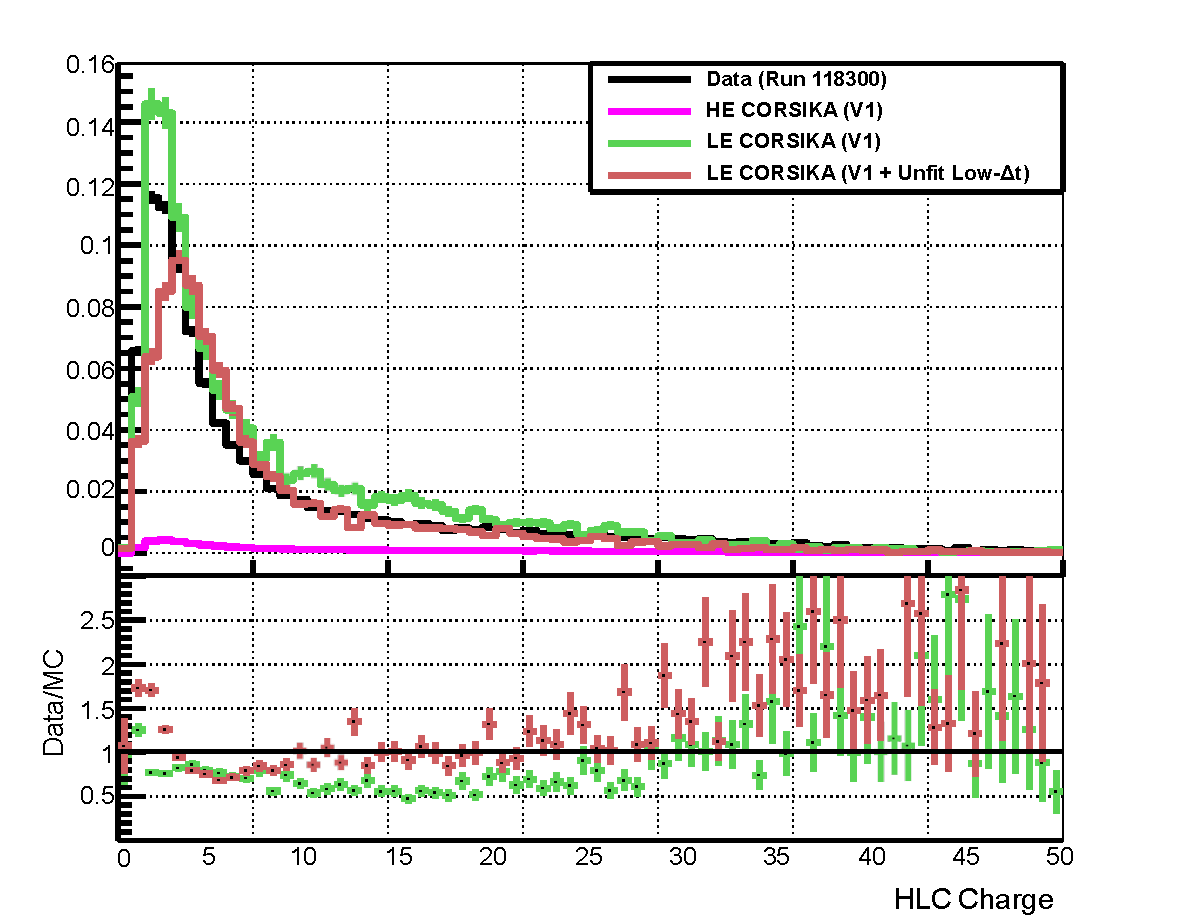
\includegraphics[width=0.45\linewidth]{old_HLC_Charge.pdf} \\
  \small (\textbf{\color{ctcolormain}a}) HLC Charge in DeepCore Events
\end{tabular} \hspace{2pt}
\begin{tabular}[b]{c}
  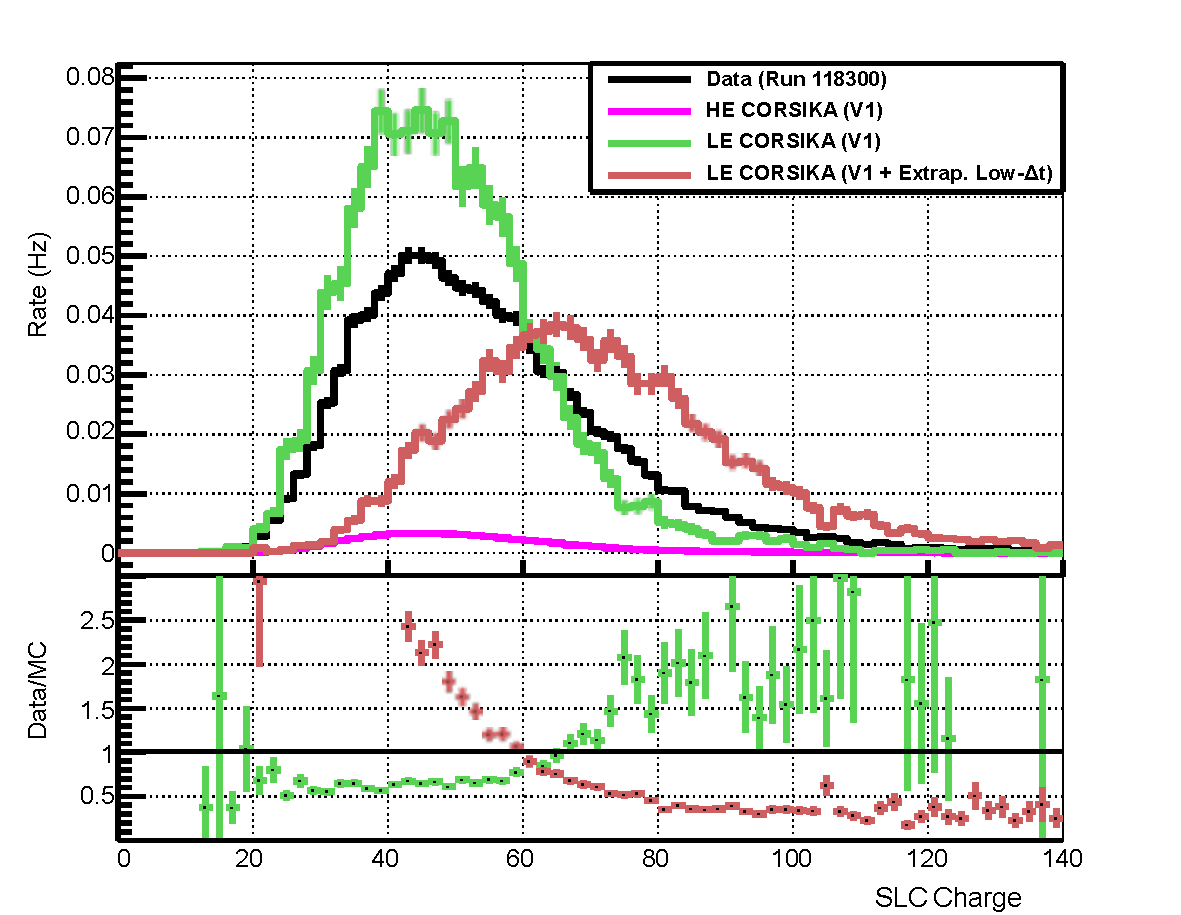
\includegraphics[width=0.45\linewidth]{old_SLC_Charge.pdf} \\
  \small (\textbf{\color{ctcolormain}b}) SLC Charge in DeepCore Events
\end{tabular}
\caption{The total amount of charge on DOMs satisfying the (a) HLC and (b) SLC criteria described in Section~\ref{subsec:LC}. The distribution from 8 hours of data (black) is shown compared to a sample of CORSIKA muons at low-energy (600 GeV $\leq E_{primary} \leq$ 100 TeV) and high energy (100 TeV $\leq E_{primary} \leq$ 100 EeV). Unlike in Figure~\ref{fig:uncalibrated_nchannel}, the charge distributions using the low-dt extension to Vuvuzela shows large disagreements with data. This is most visible in the SLC charge distribution.}
\label{fig:uncalibrated_charge}
\end{figure}

Because the extended noise model adds hits occuring at timescales down to nanoseconds, multiple hits can occur within one waveform, leading to increased observed charge.
When the noise distribution is extended below 2 microseconds, the tail of the distribution falls into the ATWD window of 322 nanoseconds, increasing the charge of noise hits in HLC DOMs.
Furthermore, some fraction of the hits in a burst of correlated noise occur within the three bins recorded from the FADC for SLC hits.
The result is that SLC hits due to noise no longer occur as single-photoelectron pulses, as is the case when noise hits are rare at the 10 nanosecond timescales, but as an integration of multiple single pulses.
Such an effect would be most visible in the charge distribution of SLC DOMs, which are more likely to be due to noise hits than HLC DOMs.

The total charge of DOMs associated with HLC and SLC hits was evaluated to look for this effect due to the extended noise model.
The result is shown in Figure~\ref{fig:uncalibrated_charge}.
The change in the charge is observed clearly in the SLC charge distribution, where a systematic shift is visible due to the low-dt extension.
Both the original Vuvuzela model and the extended Vuvuzela model show significant disagreement with data in the SLC charge distribution.
This demonstrated that the noise distribution at very short timescales was an important effect that deserved further attention.

\begin{figure}[h]
\centering
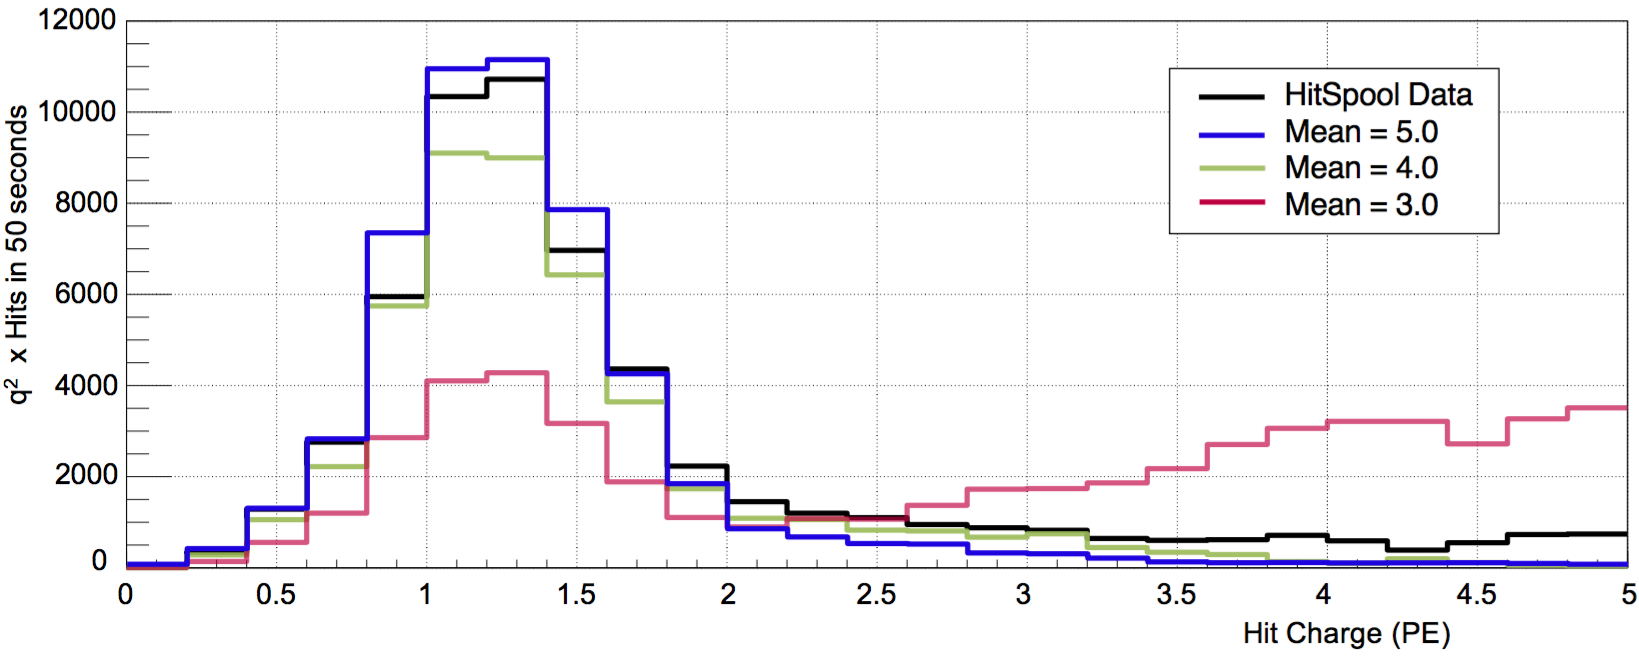
\includegraphics[width=0.5\pagewidth]{lowdt_charge_effects.png} 
\caption{The effect of changing the noise distribution parameters on the charge. Note the scale of the y-axis, which is scaled in order to emphasize the effect. Here, the gaussian mean is shifted from "5" (100 microseconds) to "3" (1 microsecond). All other parameters are held constant. By moving the correlated noise distribution to shorter timescales, more of distribution falls into one FADC bin, increasing the charge output for each launch. }
\label{fig:lowdt_effect_charge}
\end{figure}

The observed effect of the low-dt extension on the SLC charge distribution indicates that the distribution is sensitive to the region below 2 microseconds.
The charge distribution of each DOM may therefore be used in the fitting procedure in order to characterize the low-dt end of the noise timing distribution.
The effect, demonstrated in Figure~\ref{fig:lowdt_effect_charge}, allows the investigation of a part of the distribution unavailable in previous fits.

\label{sec:vuvuzela_fitting}
\section{Updating the Fitting Code}
The effect of the low-dt extension on the charge distributions indicated the potential for improvement in the noise model distribution.
New calibration fits for the updated the noise model, referred to as \emph{Vuvuzela V2} fits, were planned to include this extension for all DOMs.

With the opportunity to refit, a number of additional improvements were implemented.
The afterpulsing peak at 9 microseconds was explicitly included in the fitting code.
To account for the variability in the strength of the peak, a scale factor for the afterpulsing was included in the Vuvuzela V2 fits.

In order to include the effect of atmospheric muons, a set of Polygonato CORSIKA.
The Polygonato model was selected due to the natural weighting scheme of the output files, allowing continuous simulation of the detector.
Simulated files were divided into 10 microsecond long events (\emph{long-frame} events), each containing multiple muons.
The simulation was halted after photon propagation, giving a collection of muons without detector noise and effects applied.

\begin{landscape}
\centering
\begin{figure}
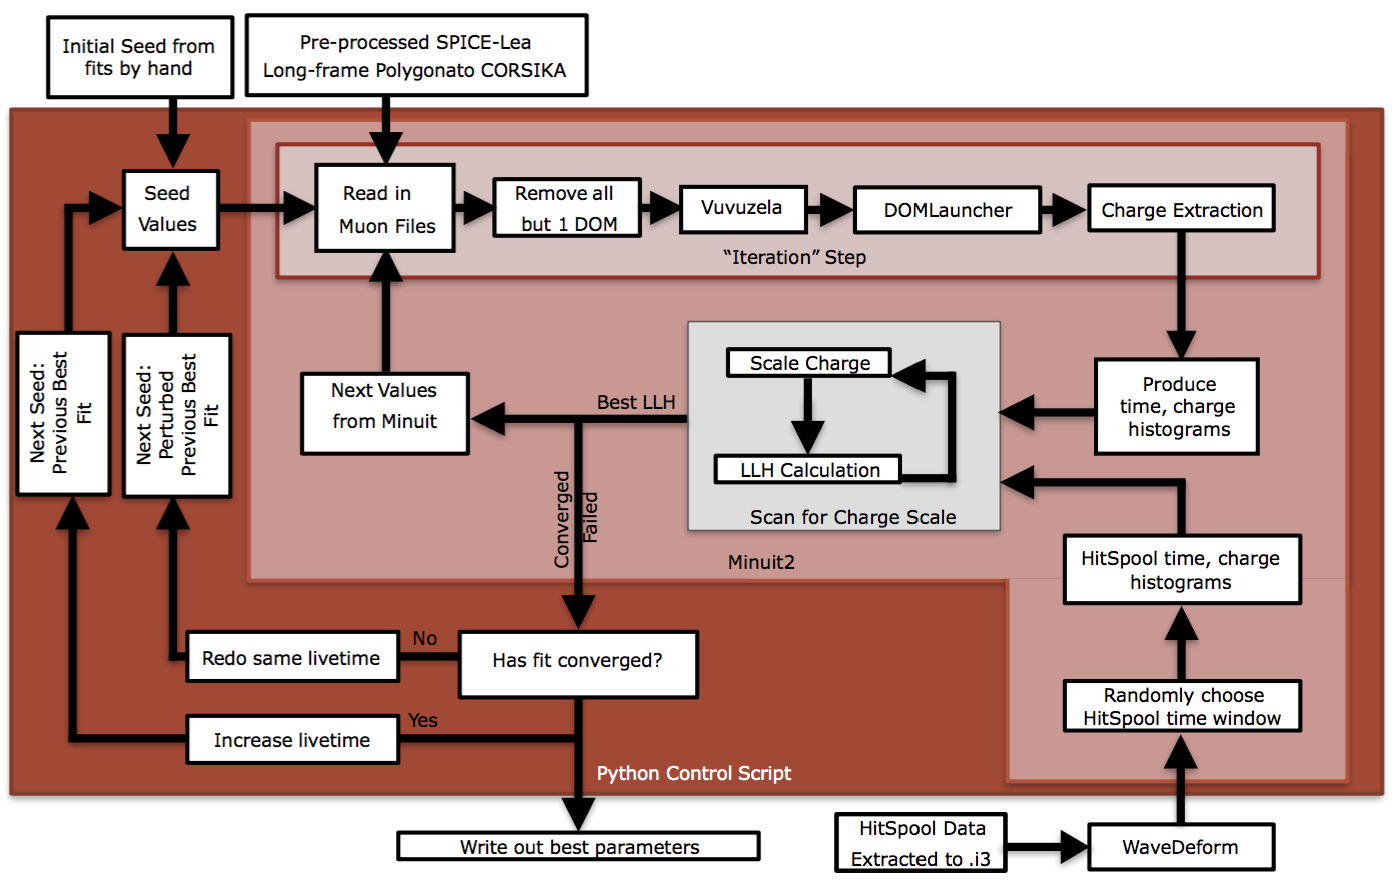
\includegraphics[height=0.8\textwidth]{fit_flowchart.png} 
\caption{A schematic diagram of the process used in the Vuvuzela V2 calibration fit.}
\label{fig:fit_flowchart}
\end{figure}
\end{landscape}

The fitting process, described schematically in Figure~\ref{fig:fit_flowchart}, is divided into several parts. 
The code started with untriggered detector data as well as the produced long-frame CORSIKA events. 
The fit included a total of six explicit parameters: the five parameters from the original Vuvuzela model as well as a scale factor for the afterpulsing.
Later investigations led to the introduction of a charge scale parameter to account for systematic differences between the data and simulated charge.
Seeds for each parameter were taken from the Vuvuzela V1 calibration fits from 2012.
Fits were performed for each DOM in parallel.

For each iteration, the long-frame CORSIKA files were filtered to remove information on all DOMs not currently being fit.
The noise and detector simulation were applied using the current parameter set for the iteration.
Charge extraction from the waveforms was performed using standard IceCube tools.
After the simulation for a given set of parameters, histograms were produced for untriggered data and simulated hits.
As in the previous fits, the time between subsequent hits is used as the primary observable of the noise behavior.
In addition, the observed charge on the DOM is used as a second observable.

\begin{figure}[h]
\centering
\begin{tabular}[b]{c}
  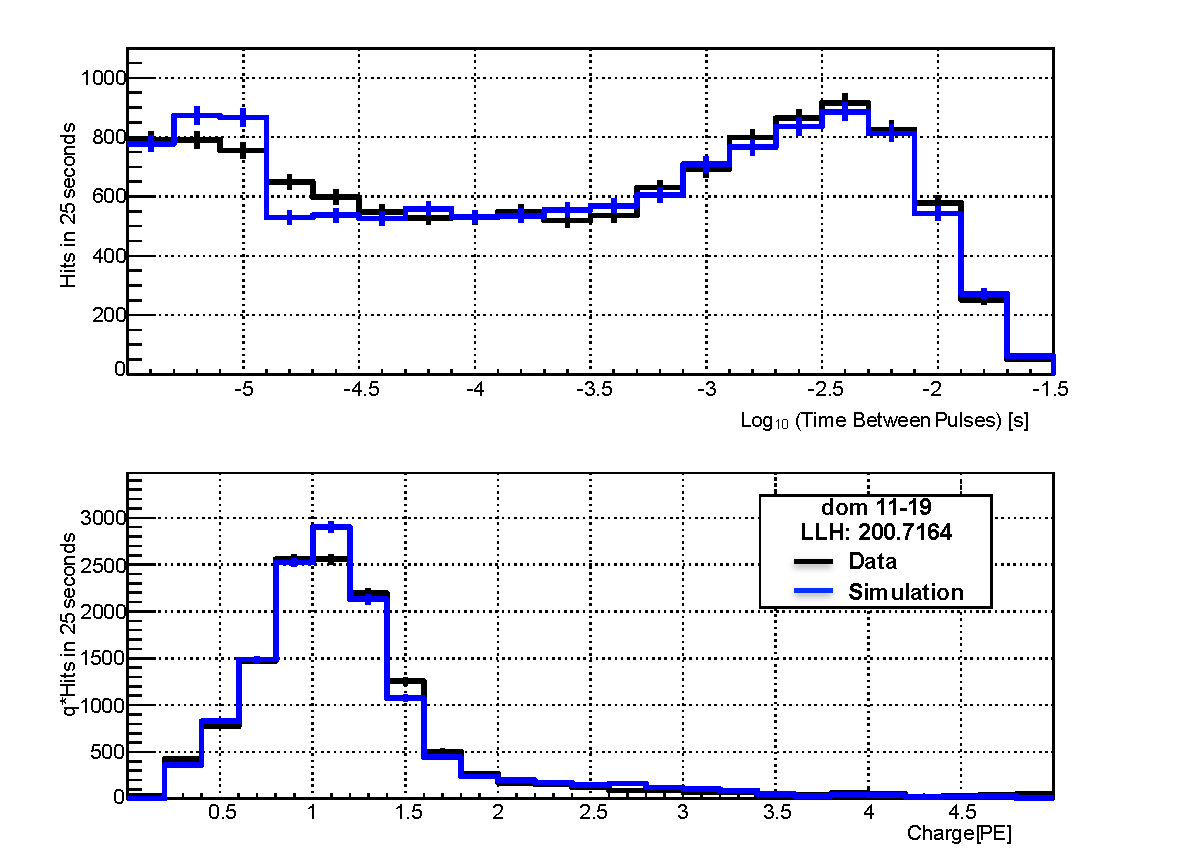
\includegraphics[width=0.45\linewidth]{new_dom_11-19.pdf} \\
  \small (\textbf{\color{ctcolormain}a}) DOM 11-19
\end{tabular} \hspace{2pt}
\begin{tabular}[b]{c}
  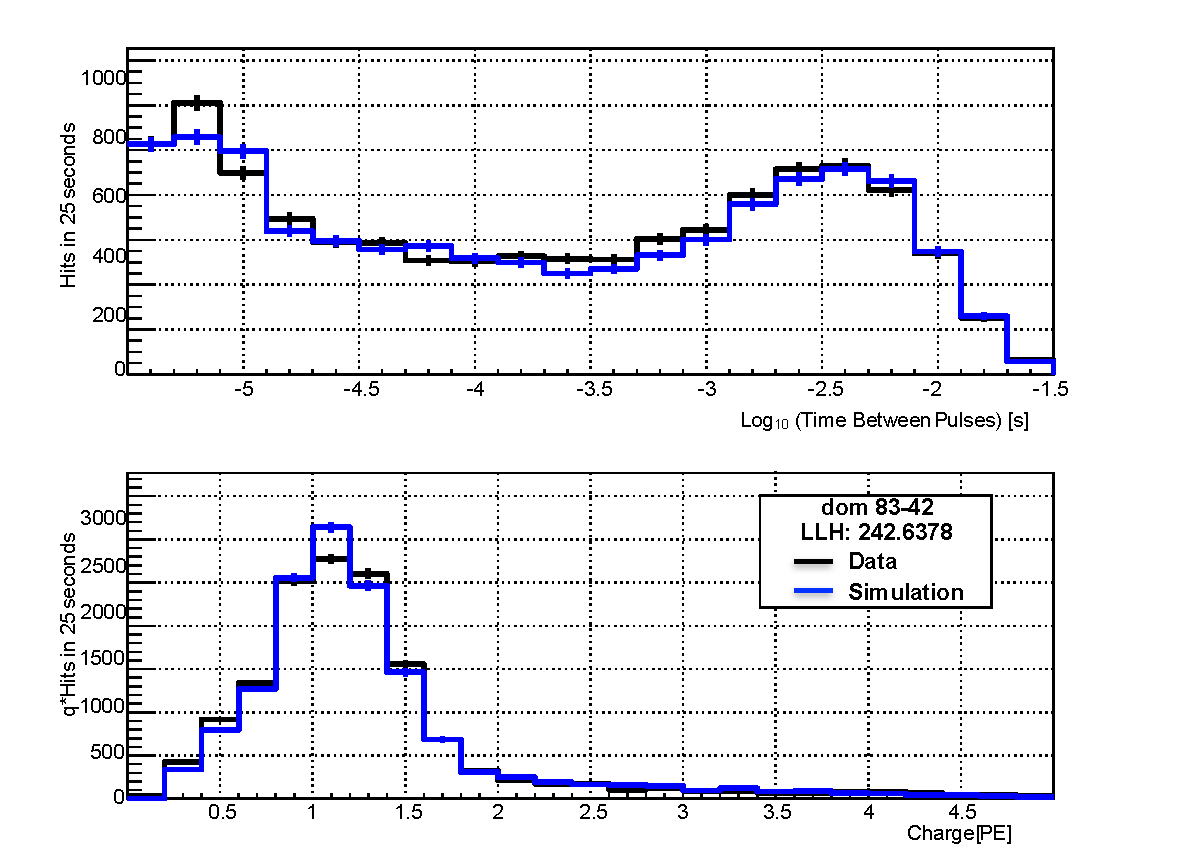
\includegraphics[width=0.45\linewidth]{new_dom_83-42.pdf} \\
  \small (\textbf{\color{ctcolormain}b}) DOM 83-42
\end{tabular}
\caption{Two examples of the new calibration fits for the Vuvuzela V2 model. The distribution of the time ("dt") between hits is shown on top. The distribution of charge is shown on the bottom. Note the y-axis of the charge distribution. In black, untriggered detector data is shown. The Vuvuzela V2 model is shown in blue. The new fits shown good agreement in both time and charge distributions.}
\label{fig:new_vuvuzela_fits}
\end{figure}

The range of the histograms, from 6 microseconds until 1 second in the time and 0-5 photoelectrons in charge, provides sensitivity to the full range of the noise distribution.
The distributions for DOMs 11-19 and 83-42 are shown in Figure~\ref{fig:new_vuvuzela_fits}.

Using the two distributions, a Poisson binned likelihood is formed.
With the simulation in bin $i$ of histogram $j$ denoted by $f_{ji}$ and the data hits in the same bin denoted by $d_{ji}$ and ignoring normalization constants, the log-likelihood takes the form

\begin{equation}
	LLH = \sum_j \sum_i^{\mathtt{nbins}_j} d_{ji} \mathtt{Log}(f_{ji}) + f_{ji}
\end{equation}

The negative log-likelihood, $-LLH$ is minimized as a function of the fit parameters using iMinuit, a python wrapper for the minuit2 package \cite{iminuit-code, iminuit-paper}.

High charges from noise hits were rarely produced, limiting the effectiveness of the fitting strategy.
To provide more weight to high charges, the histogram of the charges was weighted by the value of the observed charge.
This reduces the weight of very low charge launches, but increases the weight of higher charges.

Additional work showed that the charge distributions between data and simulation demonstrated disagreement in the charge distributions. 
This disagreement, due to miscalibration of the SPE peak in data, was accounted for by introducing a scale factor applied to the charge in simulation as a free parameter in the fit.
The charge scaling applied to the simulated hits after detector simulation.
To limit the computational complexity of the added parameter, the minimization over this charge scale factor is performed independently without resimulation.
The form of this charge scale parameter assumes that the difference is a calibration issue in the data rather than a simulation problem.
This has been shown to be the case, with an updated charge calibration now applied to data at final level.

The previous calibration attempts explicitly avoided fitting the behavior below 10 microseconds.
In particular, it was noted that mismodeled afterpulsing behavior could lead to biased results in the noise parameters.
The default value in simulation, assumed to be 5.93\% for all PMTs, failed to take into account variations in the effects on each individual DOM.
In the updated fit, the afterpulsing behavior has been investigated for each PMT by including an overall scale factor on the afterpulsing probability.

Late pulses, produced by electrons which backscatter to previous dynodes during the multiplication process, were also investigated for their effect on the goodness-of-fit in the noise distributions.
These pulses occur at timescales of 50-200 nanoseconds and therefore are outside of both the SLC charge and timing distribution window.
The late pulsing behavior was found to have a negligible impact due to both the rarity of late pulses as well as the lack of detailed information to constrain the distribution.

The effect of the afterpulsing parameter allowed some fits to fall into a poor local minimum. 
The degeneracy between parameters led to a local mimina from which the minimizer could not escape.
In these cases, the probability of observing an afterpulse following a photoelectron would be moved from 5.6\% to the unrealistically high value of 20\%. 
This forced the gaussian mean of the Vuvuzela V2 model to move toward higher values and the gaussian sigma value to become unrealistically large.
These fits were discovered by eye when looking at the best fit value of the afterpulsing probability, with a distinct population appearing due to this behavior.
In order to constrain the fit to more realistic values, bounds were added to both the log-normal mean and afterpulsing probability for DOMs where fits showed abnormal behavior. 
DOMs with particularly strong afterpulsing peaks visible by eye in data were discovered.
These DOMs were allowed to fit beyond the new boundary.

Due to the computational power required to produce large amounts of effective livetime at each iteration of the fitting process, a tiered approach was employed.
Initial fits were seeded with the previous noise parameter fit values obtained in 2012.
For these events, a coarse choice of binning both the timing and charge distributions and short effective livetime of just one minute were used.
In addition, a weak tolerance value was used, allowing the minimizer to converge quickly to a reasonable minimum.

When the first tier completes the minimization process, the fit is restarted with a larger effective livetime, more bins, and a stronger tolerance using the best-fit parameters.
The second tier used a 5 minute effective livetime, increasing the simulation time per iteration by a factor of 5.

The third and final tier increased the effective livetime to 10 minutes and again increased the number of bins.
The final tier of minimization was the most computationally intensive and required between three and four weeks per DOM. 

The fitting process for each tier continued until the minimization either converged or failed.
Failure could occur due to electronics issues, such as computing cluster downtime, or due to a limit of 10000 iterations set in the minimizer to prevent issues with maximum processing time available on the computing cluster. 
In the case of a failure, the fitting tier was restarted with a new set of seed values.
The new seed values were selected from a gaussian distribution centered on the previous seed with a width of 5\%. 
The fit was then restarted.
This process was continued until the third tier was complete for all DOMs.

\label{sec:vuvuzela_newfits}
\section{Results of New Noise Fits}
New calibration fits were completed over the course of two months for nearly all DOMs in the IceCube detector.
String 25 and DOMs previously disabled due to malfunction are absent from the untriggered data, taken in 2014, used here and were therefore left unfit.
The parameters for string 25 were selected using the average of all other fits.


\begin{figure}[h]
\centering
\begin{tabular}{cc}
  	 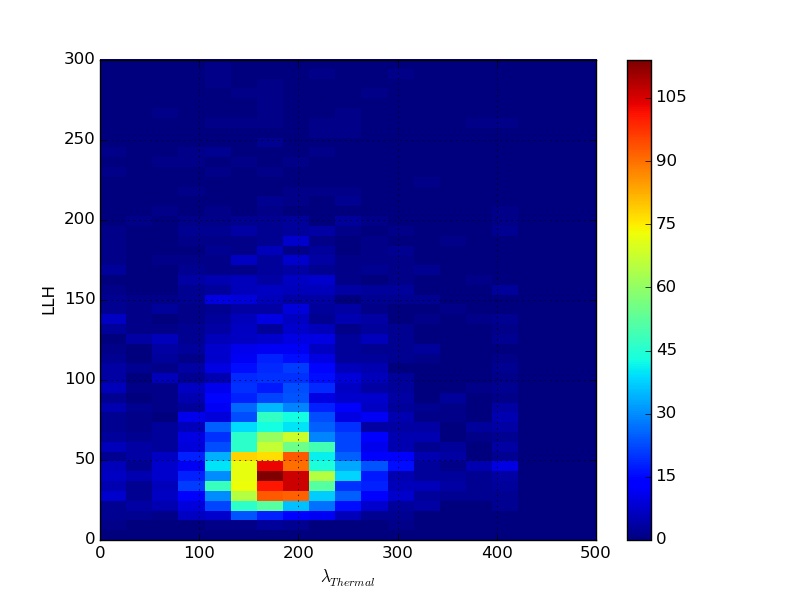
\includegraphics[width=0.45\linewidth]{llh_vs_thermal.png} &
	 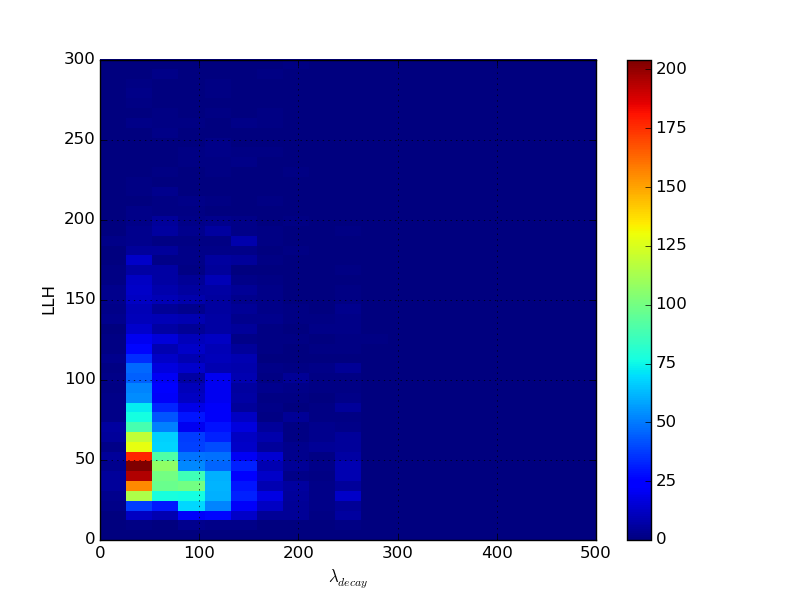
\includegraphics[width=0.45\linewidth]{llh_vs_decay.png} \\
 	 
 	 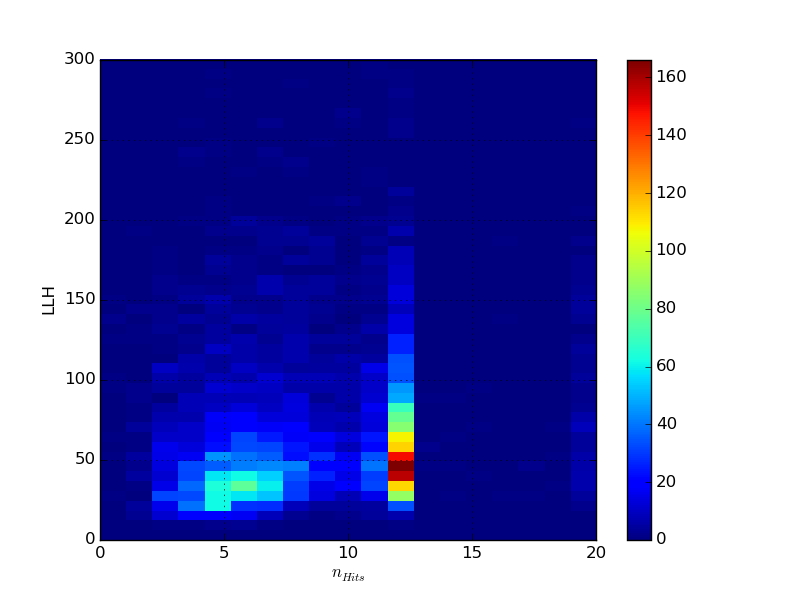
\includegraphics[width=0.45\linewidth]{llh_vs_nhits.png}  &
	 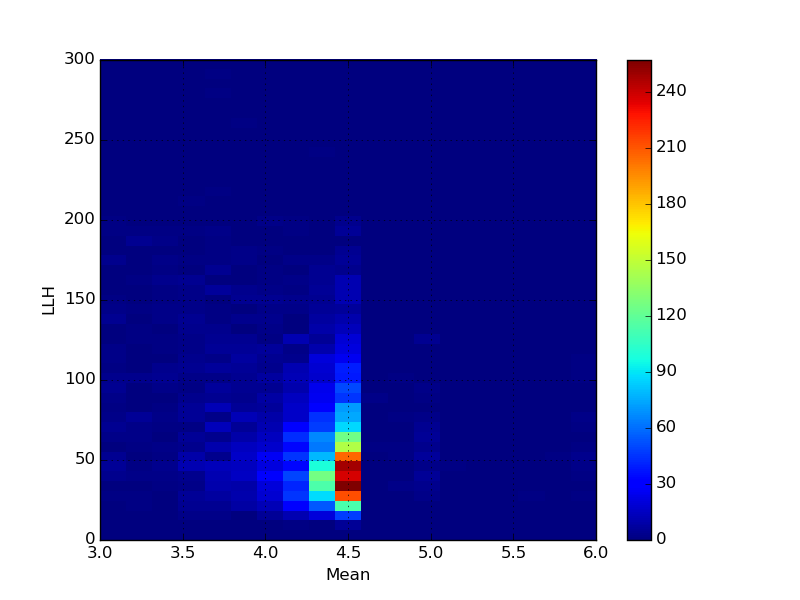
\includegraphics[width=0.45\linewidth]{llh_vs_mean.png} \\

	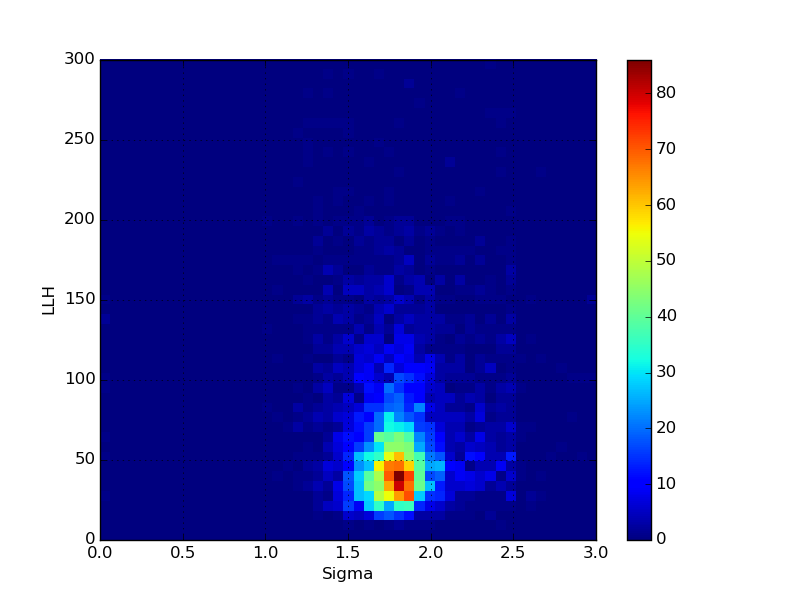
\includegraphics[width=0.45\linewidth]{llh_vs_sigma.png}  &
	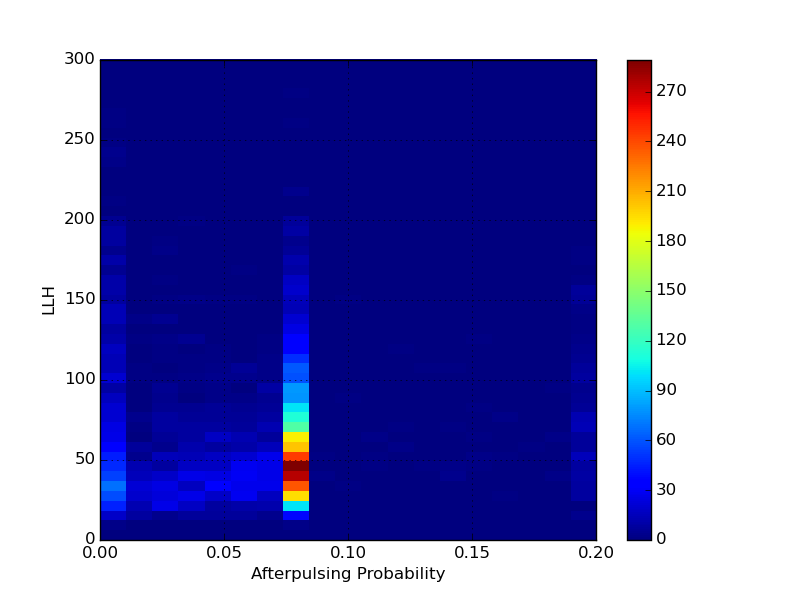
\includegraphics[width=0.45\linewidth]{llh_vs_afterpulsing.png} \\
\end{tabular}
\caption{The distributions of each new fit parameter in the Vuvuzela V2 model. The colorbar scale shows the number of DOMs in each bin. The effects of fit bounds are visible in most distributions except for the thermal noise rate and the width of the log-normal distribution describing the non-Poissonian noise.}
\label{fig:vuvuzela_params_vs_llh}
\end{figure}

The Vuvuzela V2 fits were checked after convergence in Figure~\ref{fig:vuvuzela_params_vs_llh} and Figure.
One notable feature is the number of DOMs with afterpulsing at and beyond the fitter boundary.
The likelihood values associated with these fits, however, appear to be consistent with other fits.
Due to a planned overhaul of the afterpulsing simulation, the fit values of the afterpulsing probabilities have not been adopted for simulation.
Therefore, no further investigation of the probabilities has been persued.

\begin{figure}[h]
\centering
\begin{tabular}{cc}
  	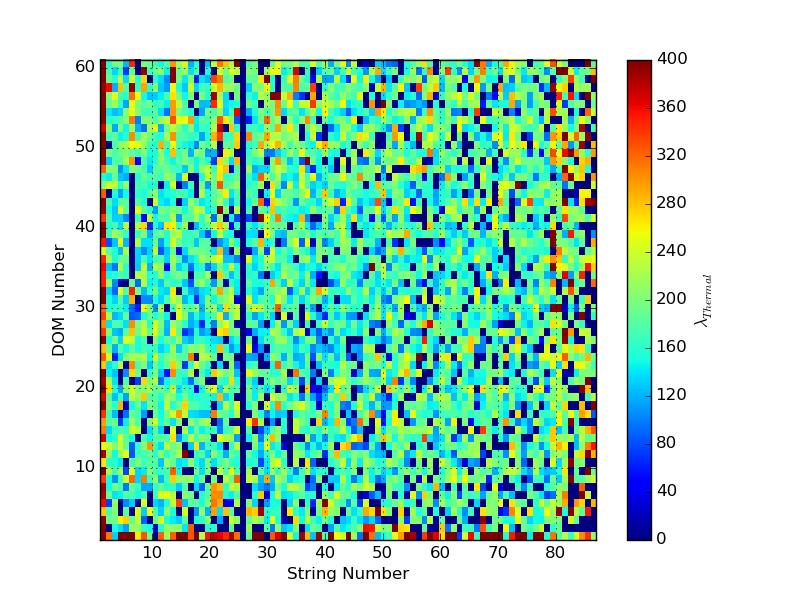
\includegraphics[width=0.45\linewidth]{thermal_occupancy.png} &
	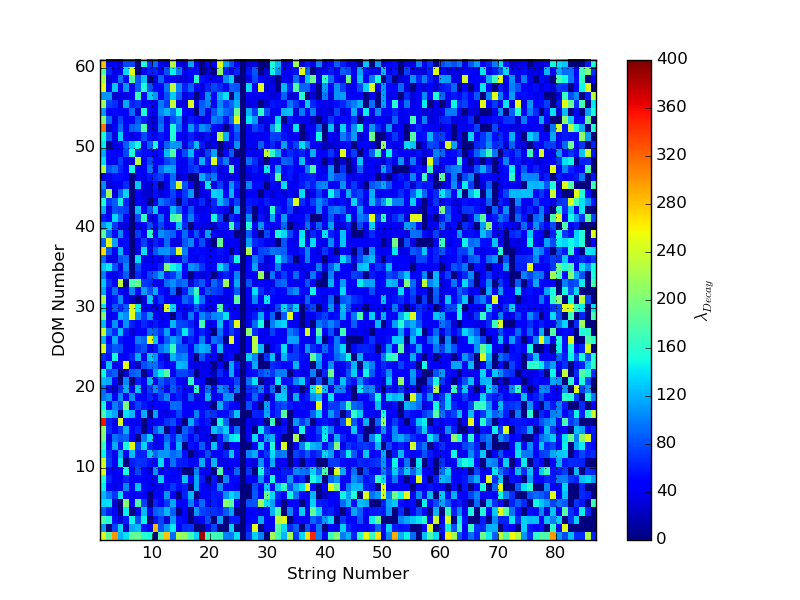
\includegraphics[width=0.45\linewidth]{decay_occupancy.png} \\

  	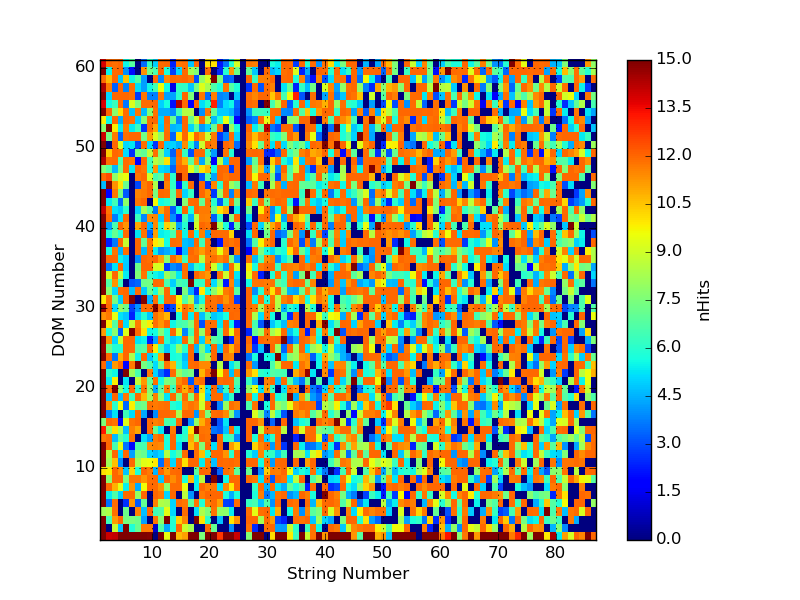
\includegraphics[width=0.45\linewidth]{nhits_occupancy.png} &
	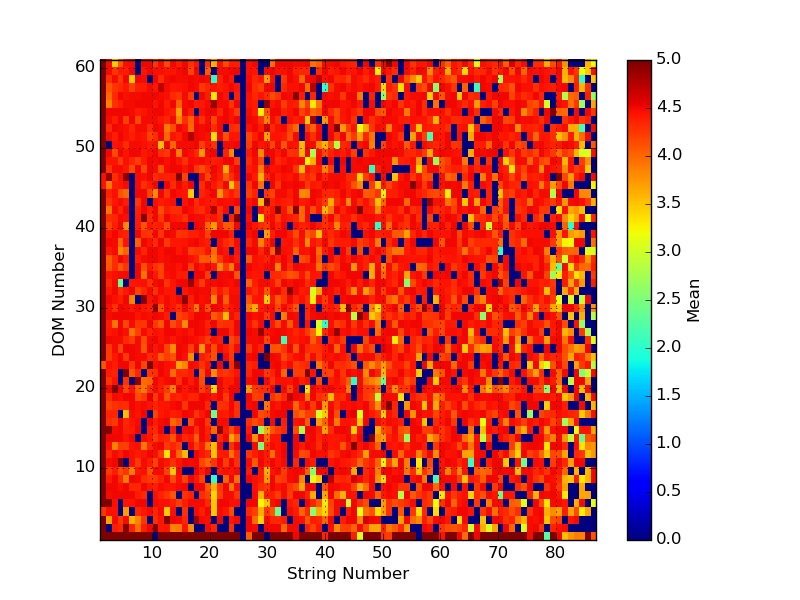
\includegraphics[width=0.45\linewidth]{mean_occupancy.png} \\

  	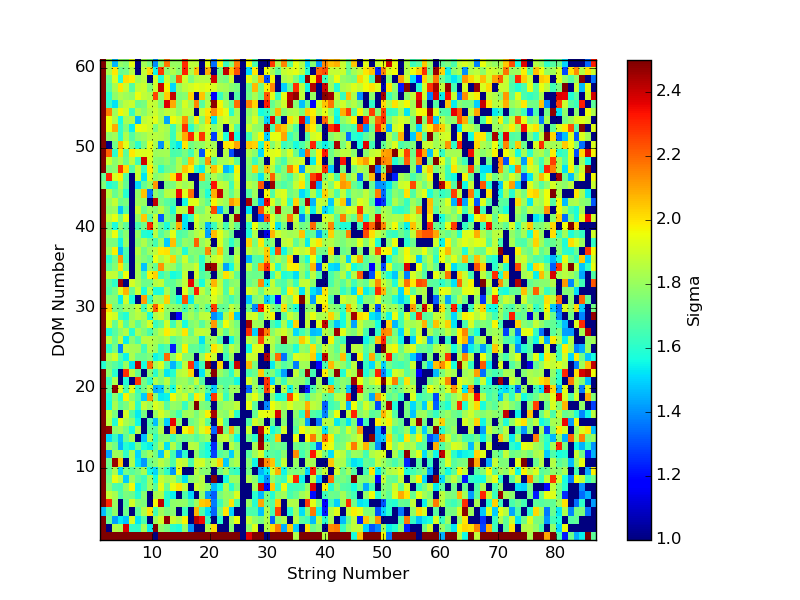
\includegraphics[width=0.45\linewidth]{sigma_occupancy.png} & 
  	\\
\end{tabular}	
\caption{The distributions of each new fit parameter in the Vuvuzela V2 model as a function of the string and DOM number. Note that the top of the detector is at the bottom of this plot. No parameter appears to be correlated with depth. DOMs on string 25 are missing from the dataset. In addition, DOMs which are disabled due to malfunction are also unavailable.}
\label{fig:vuvuzela_params_occupancy}
\end{figure}

The thermal rate is associated with the electronic noise, which should show increasing rate with increasing depth due to the rising temperature.
This effect is only weakly apparent in Figure~\ref{fig:vuvuzela_params_occupancy}.

Other parameters should be independent of depth.
As a test of the fits, each of the other parameters is plotted as a function of depth as well.
No significant correlation is observed.

\begin{figure}
\centering
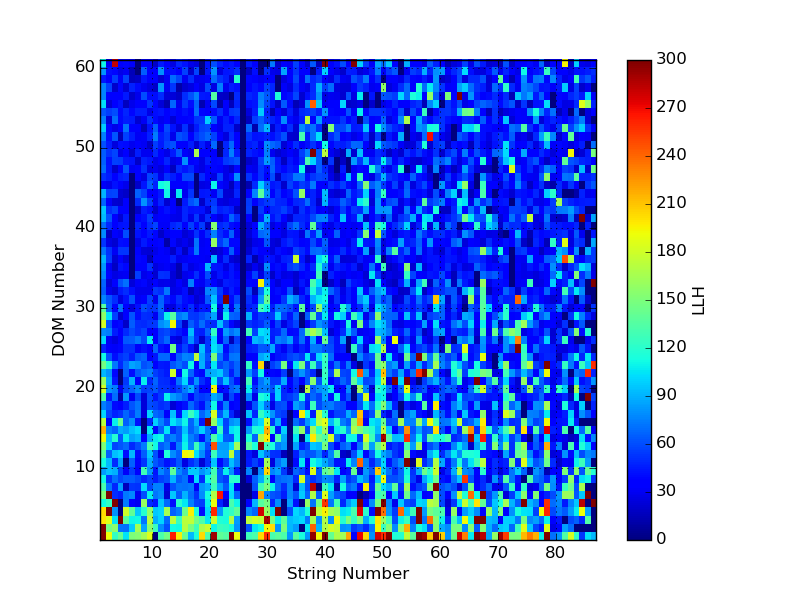
\includegraphics[width=0.9\textwidth]{llh.png} 
\caption{The log-likelihood as a function of string and DOM number for the Vuvuzela V2 fits. Note that DOM 1 is at the top of the detector and DOM 60 at the bottom. The likelihood value was expected to be independent of depth, but shows some structure. These structures are correlated with both the ice model and the muon flux.}
\label{fig:llh_vs_depth}
\end{figure}

Finally, the likelihood values should be independent of depth.
This final test, shown in Figure~\ref{fig:llh_vs_depth},  shows surprising results in at least two ways:
a 'band' structure appears in the plot. and there appears to be a depth-dependent decrease in the likelihood value, indicating that the lower part of the detector yields better fit results.
This was initially unexpected, given that the noise is an internal property of the DOM and not of the surrounding medium.

This effect occurs due to a combination of factors. 
It is worth noting that the noise measurements of each DOM are not fully independent.
The fits themselves use the long-frame CORSIKA to model the effects of muons in the untriggered data from the detector.

This leads to two subtle limitations in the fitting process.
The long-frame CORSIKA is produced with a single flux model, in this case the Polygonato model used in CORSIKA \cite{Hoerandel-Polygonato}.
Because the long-frame CORSIKA cannot be reweighted to other models, uncertainties or mismodeling in the muon flux can lead to disagreement in the fitting of noise parameters.
The muon flux decreases with increasing depth, resulting in a lower muon contamination, and consequently smaller effects from mismodeling of the muon background, for deeper DOMs. 

In addition, the long-frame CORSIKA implicitly assumes a single model of the ice for photon propagation.
Mismodeling of the scattering and absorption of the ice therefore may also give rise to disagreement in the noise calibration.
While large-scale properties of the ice are believed to be well-reproduced by the chosen ice model, SpiceLea \cite{IceCube-SpiceLea}, there will inevitably be remaining disagreements.

The net effect of these two assumptions in the muon simulation is effectively correlated with the convolution of the ice model and the muon flux.
In particular, the best fits occur where the DOM is either A) well-shielded from light due to muons by the large overburden or B) well-shielded due to large absorption in the ice.
In both cases, the contamination from light due to muons in the fitted time and charge distributions will be small, leading to a more 'pure' noise distribution that is well-fit by the Vuvuzela V2 noise model.

The sensitivity of the noise calibration procedure to underlying assumptions of both the muon flux and the absorption properties in the detector imply that little further improvement is likely without additional work on one or both issues.
Simulation of long-frame CORSIKA is, unfortunately, not possible with newer flux models at this time.
As the primary uncertainty affecting the goodness-of-fit appears to be due to the visibility and flux of the muons themselves, merely updating to a newer model of the ice will be unlikely to significantly improve the current fit parameters.

The newly calibrated low-dt Vuvuzela was provided to the IceCube simulation group in January of 2015 and quickly integrated into the low-energy simulation chain.
New neutrino, muon, and accidental noise trigger simulations were produced soon thereafter.
The updated noise model shows significantly better agreement in both the total charge distribution and the number of hit DOMs for both HLC and SLC+HLC hits.
The rate of accidental triggers improved relative to previous calibrations, with the remaining rate disagreement reduced from 50\% to approximately 15\%.
Negligible effect was observed in the low-energy neutrino events at final level for existing samples.

